\begin{figure*}[t]
\centering
\begin{subfigure}[t]{0.24\textwidth}
    \centering
    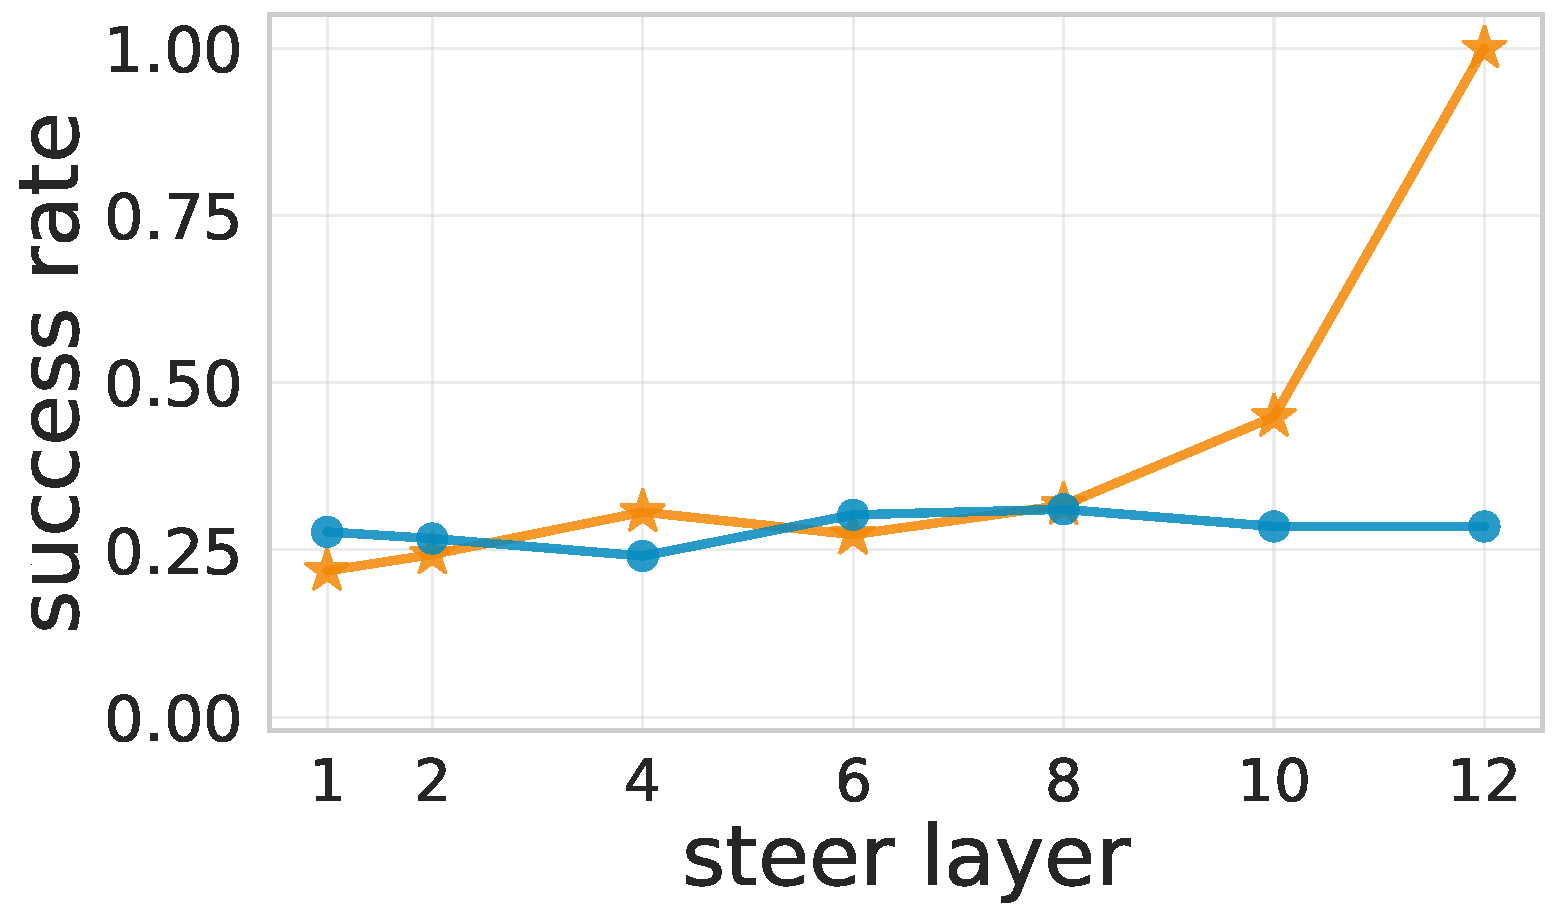
\includegraphics[width=\linewidth]{results_steer_layers/by_layer_atom_type.pdf}
    \subcaption{atom type}
\end{subfigure}\hfill
\begin{subfigure}[t]{0.24\textwidth}
    \centering
    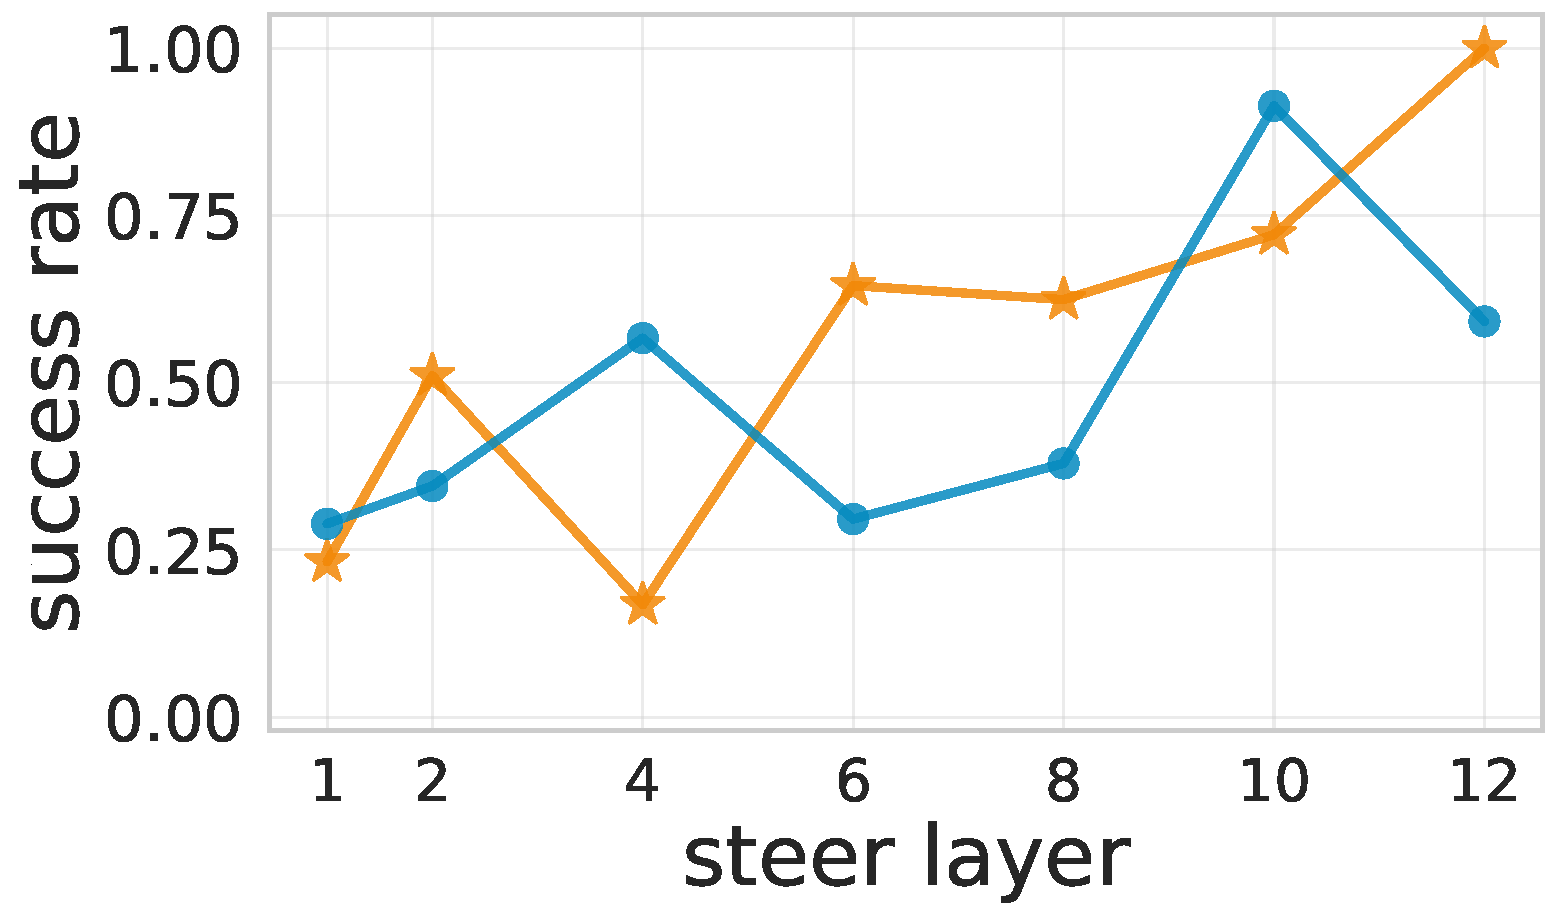
\includegraphics[width=\linewidth]{results_steer_layers/by_layer_hybridization.pdf}
    \subcaption{hybridization}
\end{subfigure}\hfill
\begin{subfigure}[t]{0.24\textwidth}
    \centering
    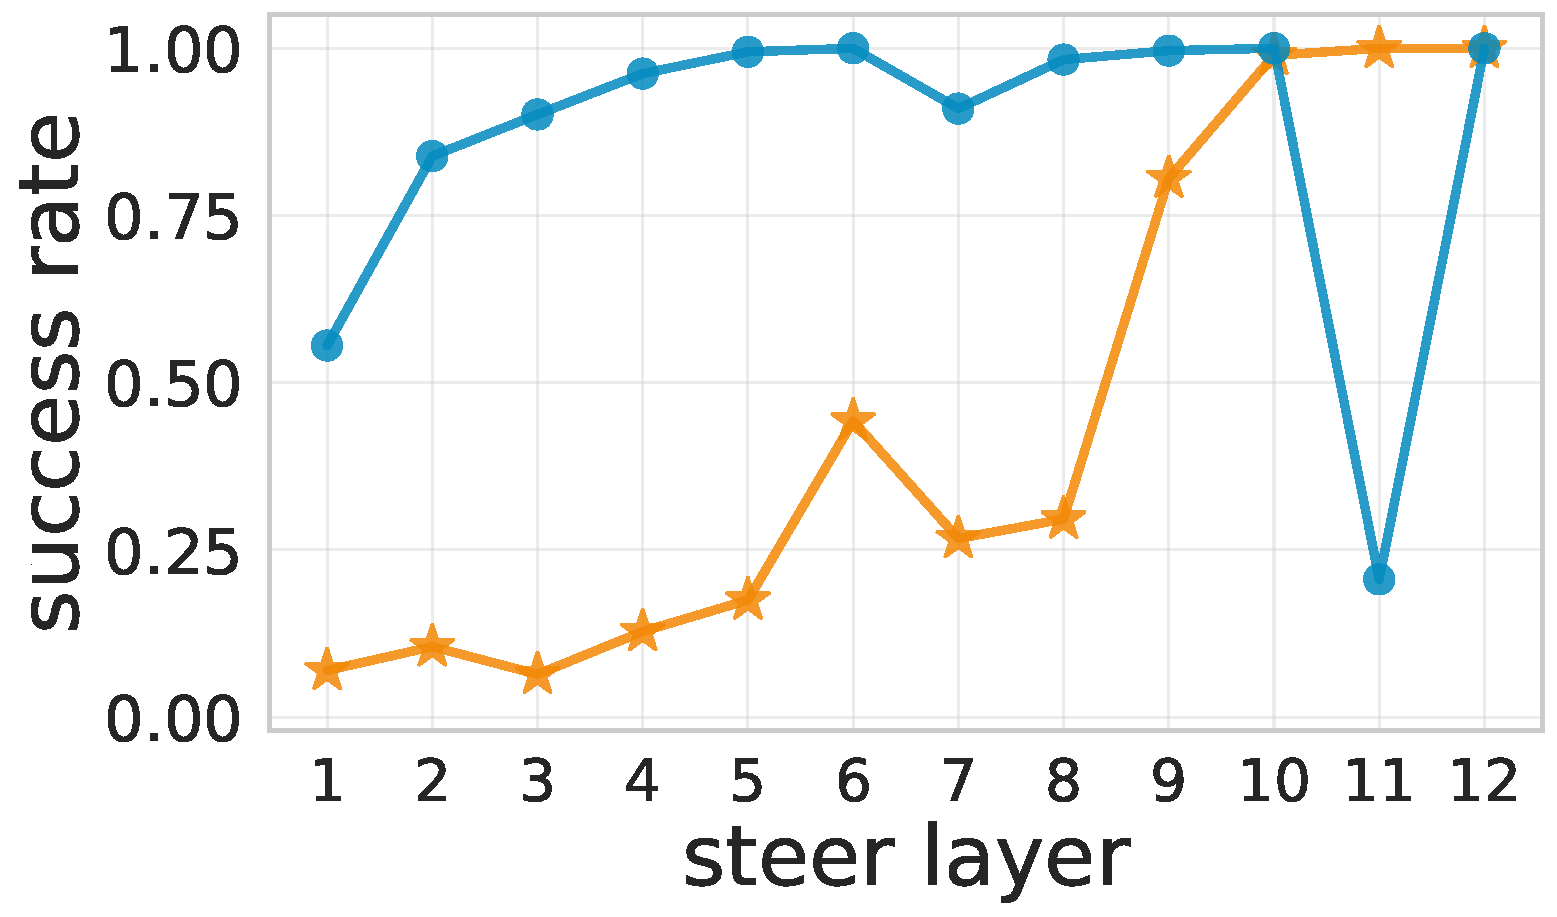
\includegraphics[width=\linewidth]{results_steer_layers/by_layer_chiral_tag.pdf}
    \subcaption{chiral tag}
\end{subfigure}\hfill
\begin{subfigure}[t]{0.24\textwidth}
    \centering
    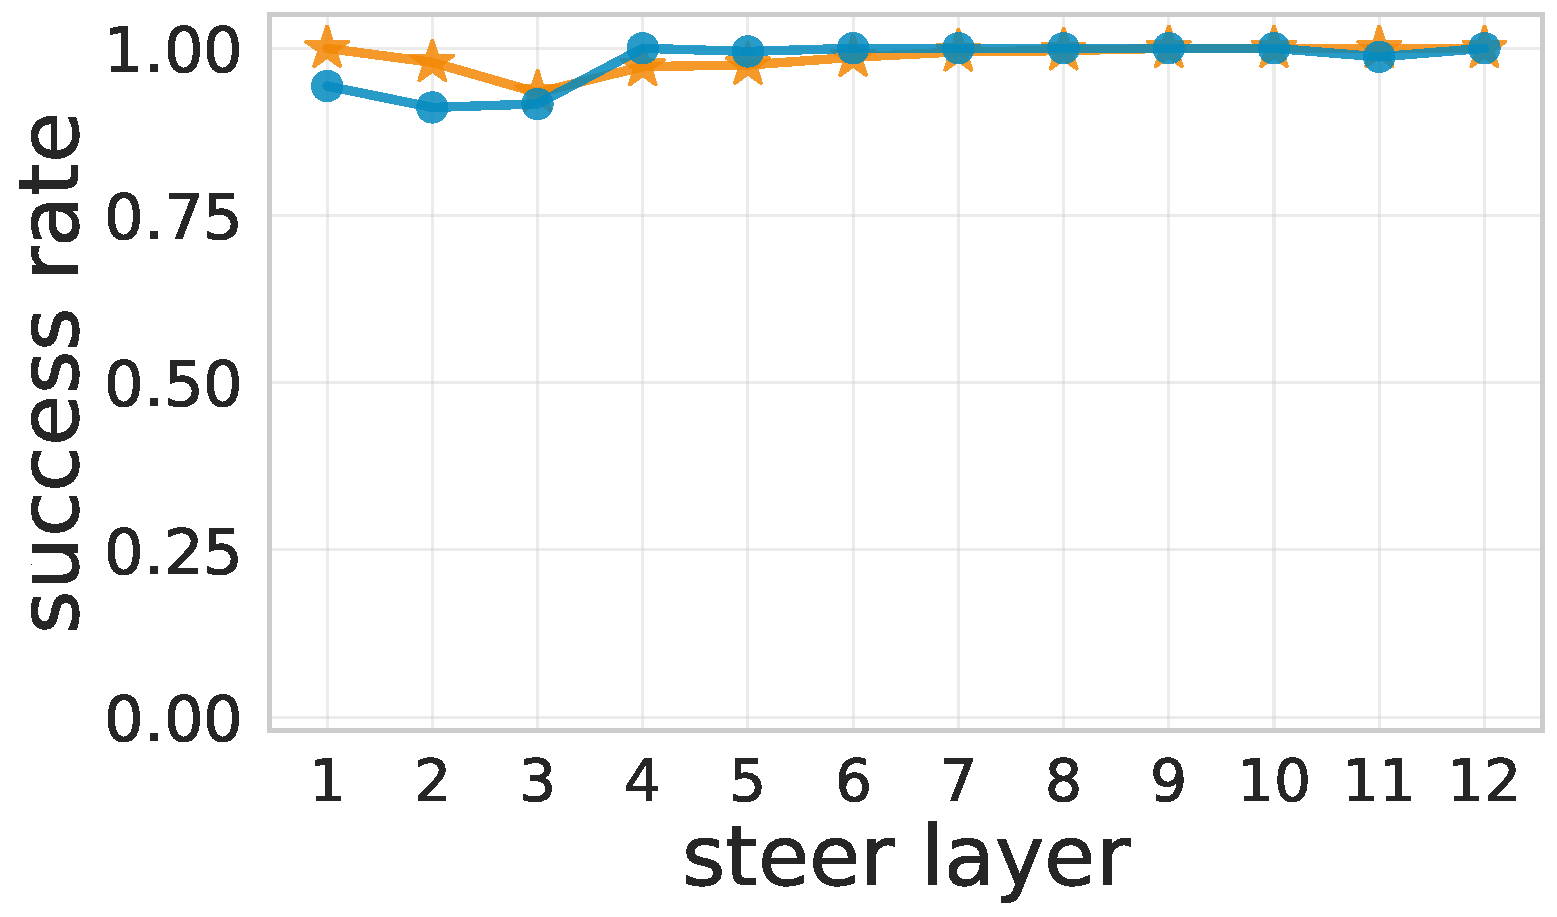
\includegraphics[width=\linewidth]{results_steer_layers/by_layer_is_aromatic.pdf}
    \subcaption{is aromatic}
\end{subfigure}
\vspace{0.6em}

\begin{subfigure}[t]{0.24\textwidth}
    \centering
    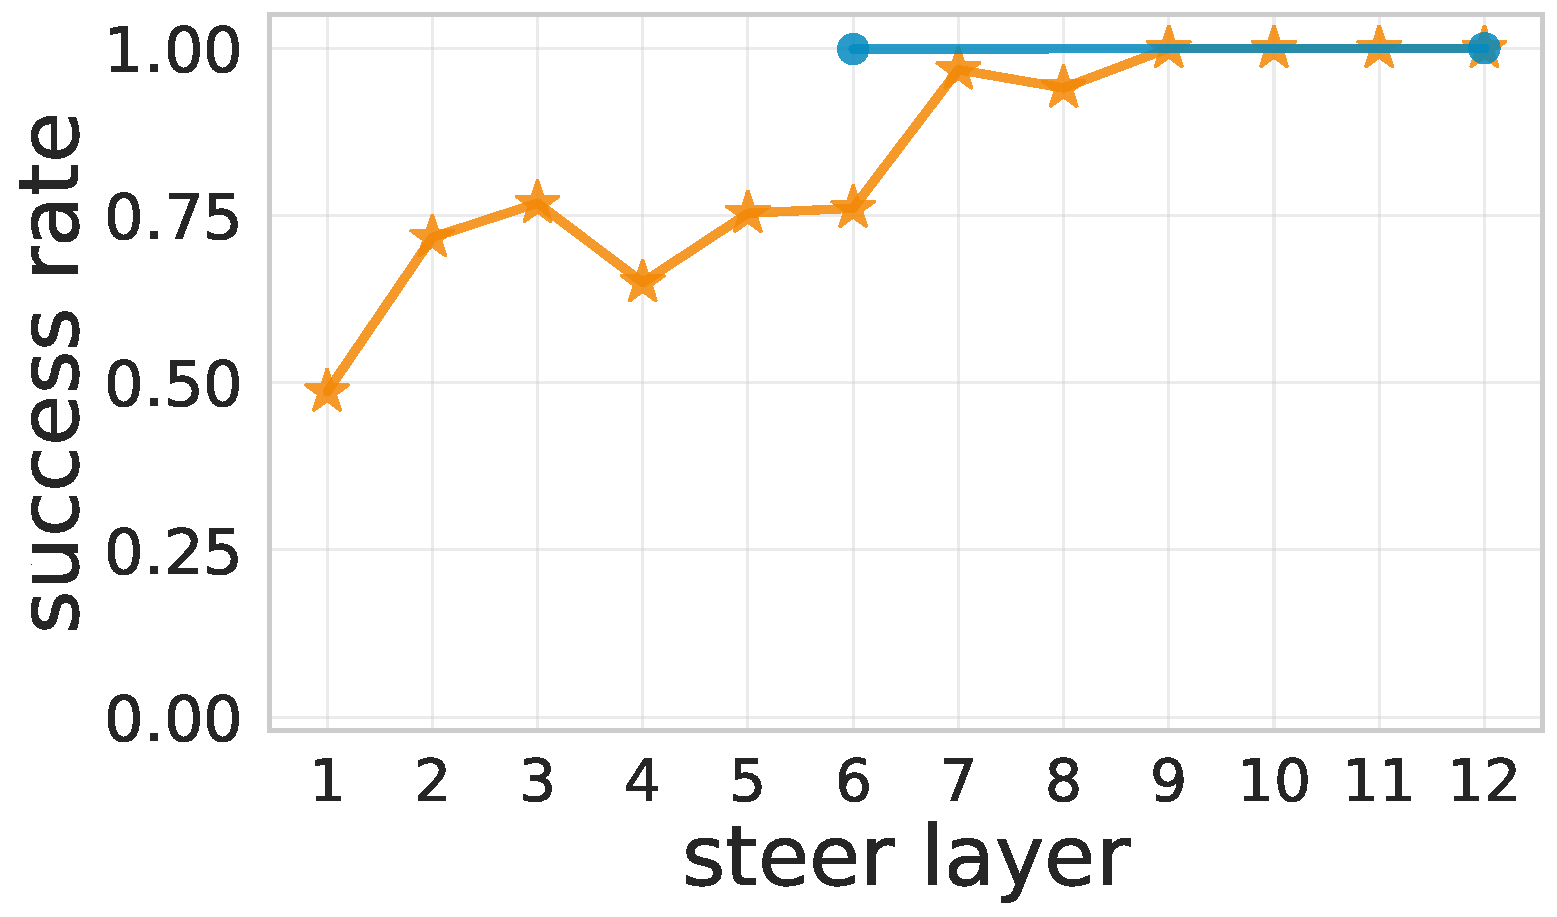
\includegraphics[width=\linewidth]{results_steer_layers/by_layer_is_in_ring.pdf}
    \subcaption{is in ring}
\end{subfigure}\hfill
\begin{subfigure}[t]{0.24\textwidth}
    \centering
    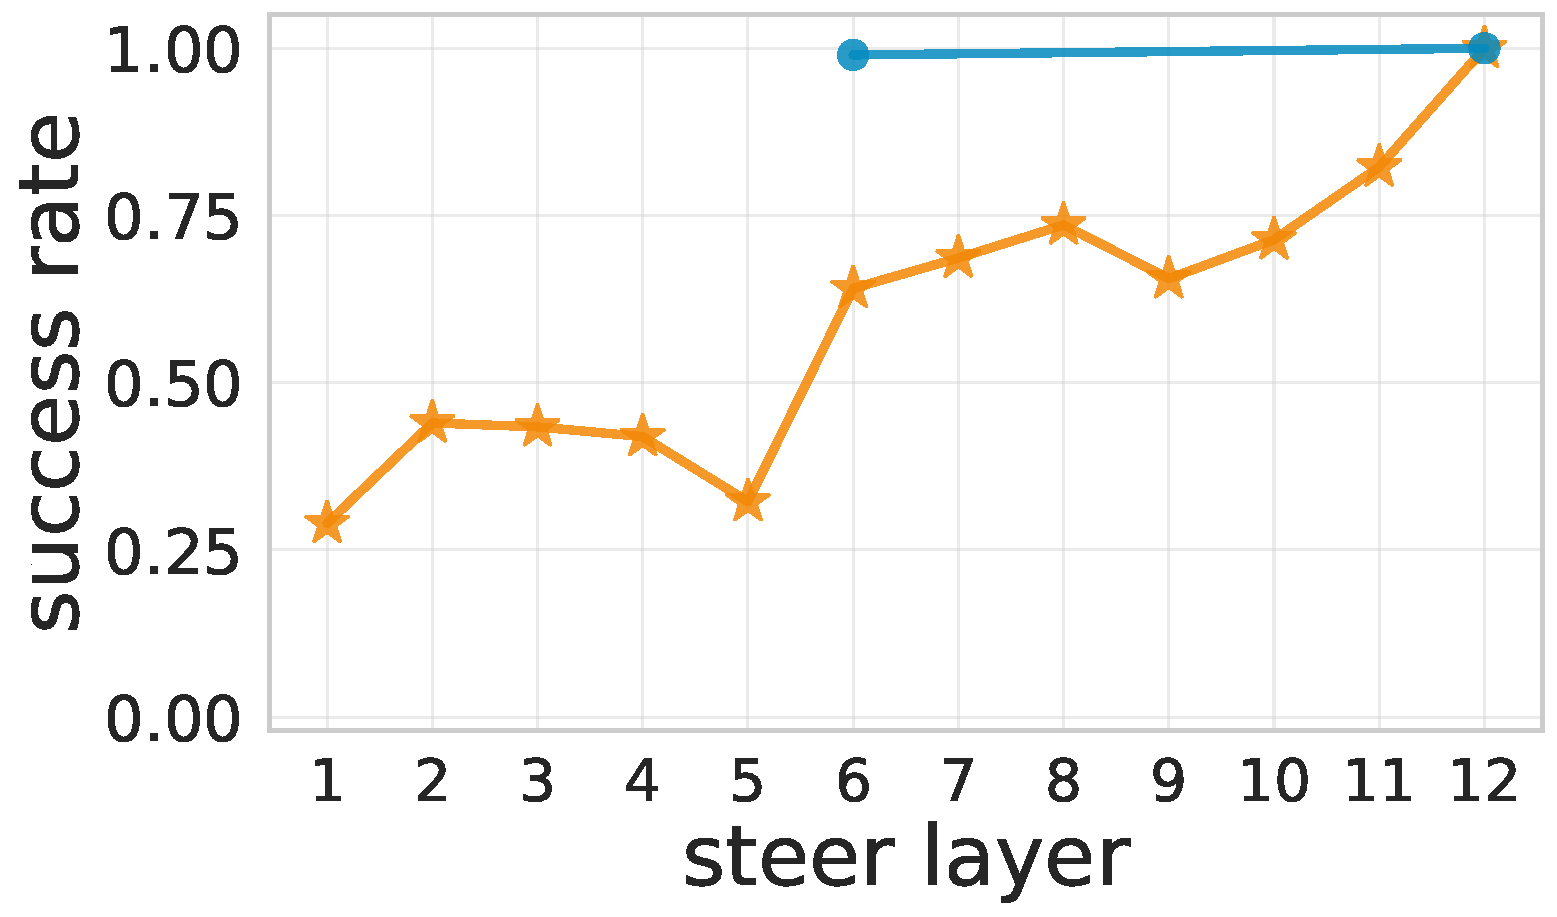
\includegraphics[width=\linewidth]{results_steer_layers/by_layer_degree.pdf}
    \subcaption{degree}
\end{subfigure}\hfill
\begin{subfigure}[t]{0.24\textwidth}
    \centering
    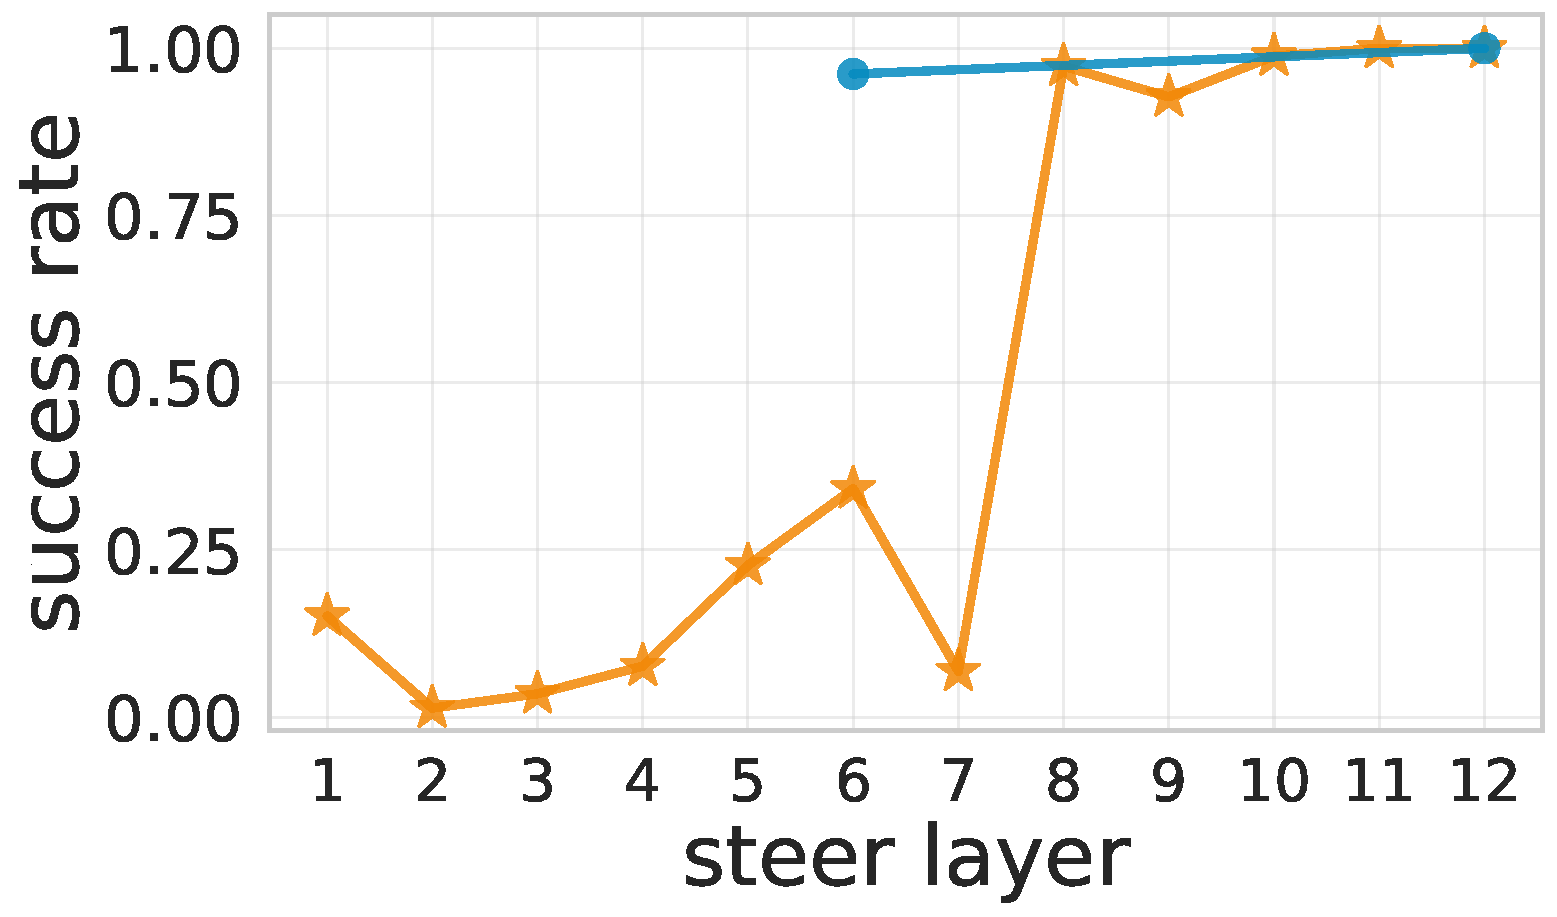
\includegraphics[width=\linewidth]{results_steer_layers/by_layer_formal_charge.pdf}
    \subcaption{formal charge}
\end{subfigure}\hfill
\begin{subfigure}[t]{0.24\textwidth}
    \centering
    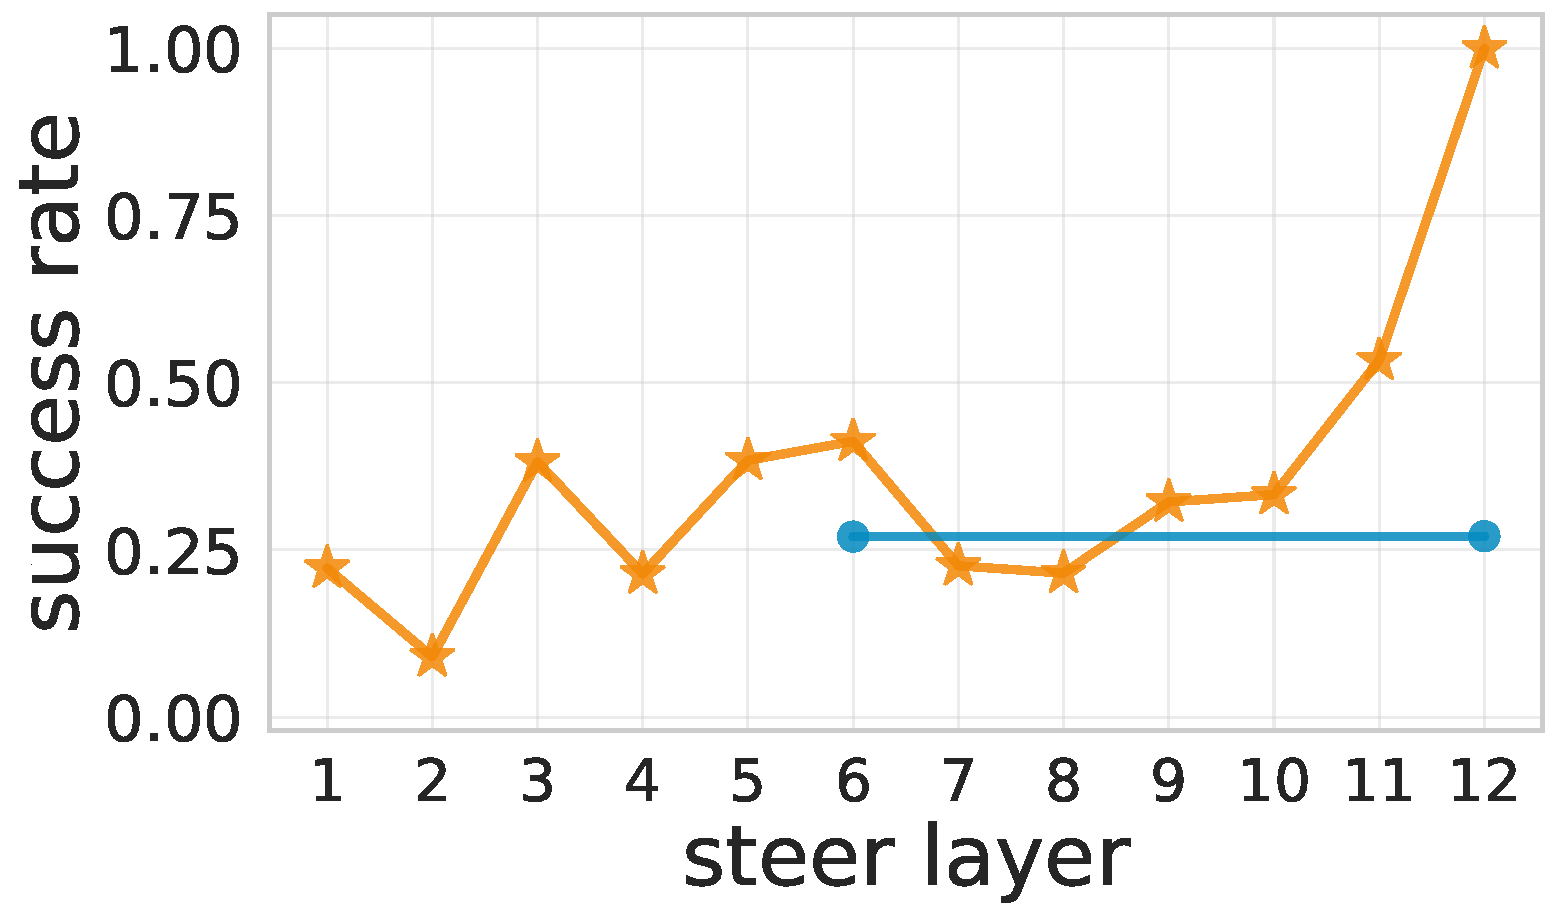
\includegraphics[width=\linewidth]{results_steer_layers/by_layer_total_valence.pdf}
    \subcaption{total valence}
\end{subfigure}

\vspace{0.4em}

\centerline{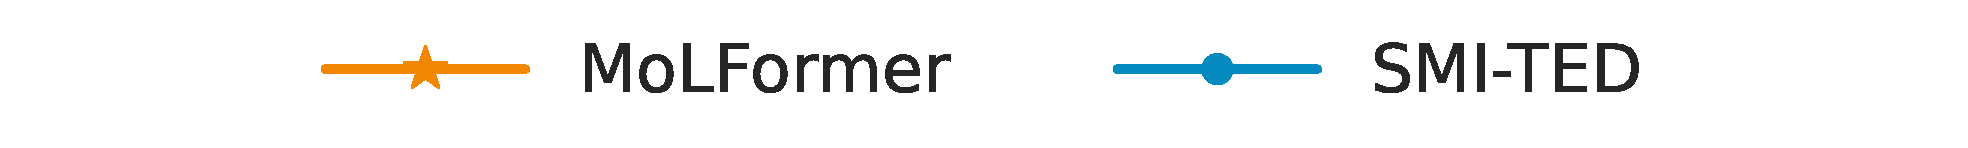
\includegraphics[width=0.5\textwidth]{results_steer_layers/by_layer_legend.pdf}}

\caption{\textbf{Intervention success rate as a function of the steer layer.} For each (task, model, layer~$\ell$) we intervene at $\ell$ along the layer-$\ell$ probe direction and read the layer-$12$ probe; the curve plots the best success rate over $\alpha$ on $200$ held-out QM9 molecules. \smi's curve is flat near~$1$ on all binary contextual tasks (ring membership, aromaticity), meaning the probed direction is a usable channel at \emph{every} depth. \molm's ring-membership curve climbs from $\sim 0.5$ at layer~$1$ to $1.00$ by layer~$9$, indicating the information is causally used only at the deepest layers despite being partially decodable throughout. Multi-class tasks (atom type, hybridization, total valence) include a probe-prototype geometry confound on the cycle target and are interpreted with that caveat in the text.}
\label{fig:steer-layer}
\end{figure*}
